\documentclass[12pt,letterpaper]{article}\usepackage[]{graphicx}\usepackage[]{color}
%% maxwidth is the original width if it is less than linewidth
%% otherwise use linewidth (to make sure the graphics do not exceed the margin)
\makeatletter
\def\maxwidth{ %
  \ifdim\Gin@nat@width>\linewidth
    \linewidth
  \else
    \Gin@nat@width
  \fi
}
\makeatother

\definecolor{fgcolor}{rgb}{0.345, 0.345, 0.345}
\newcommand{\hlnum}[1]{\textcolor[rgb]{0.686,0.059,0.569}{#1}}%
\newcommand{\hlstr}[1]{\textcolor[rgb]{0.192,0.494,0.8}{#1}}%
\newcommand{\hlcom}[1]{\textcolor[rgb]{0.678,0.584,0.686}{\textit{#1}}}%
\newcommand{\hlopt}[1]{\textcolor[rgb]{0,0,0}{#1}}%
\newcommand{\hlstd}[1]{\textcolor[rgb]{0.345,0.345,0.345}{#1}}%
\newcommand{\hlkwa}[1]{\textcolor[rgb]{0.161,0.373,0.58}{\textbf{#1}}}%
\newcommand{\hlkwb}[1]{\textcolor[rgb]{0.69,0.353,0.396}{#1}}%
\newcommand{\hlkwc}[1]{\textcolor[rgb]{0.333,0.667,0.333}{#1}}%
\newcommand{\hlkwd}[1]{\textcolor[rgb]{0.737,0.353,0.396}{\textbf{#1}}}%

\usepackage{framed}
\makeatletter
\newenvironment{kframe}{%
 \def\at@end@of@kframe{}%
 \ifinner\ifhmode%
  \def\at@end@of@kframe{\end{minipage}}%
  \begin{minipage}{\columnwidth}%
 \fi\fi%
 \def\FrameCommand##1{\hskip\@totalleftmargin \hskip-\fboxsep
 \colorbox{shadecolor}{##1}\hskip-\fboxsep
     % There is no \\@totalrightmargin, so:
     \hskip-\linewidth \hskip-\@totalleftmargin \hskip\columnwidth}%
 \MakeFramed {\advance\hsize-\width
   \@totalleftmargin\z@ \linewidth\hsize
   \@setminipage}}%
 {\par\unskip\endMakeFramed%
 \at@end@of@kframe}
\makeatother

\definecolor{shadecolor}{rgb}{.97, .97, .97}
\definecolor{messagecolor}{rgb}{0, 0, 0}
\definecolor{warningcolor}{rgb}{1, 0, 1}
\definecolor{errorcolor}{rgb}{1, 0, 0}
\newenvironment{knitrout}{}{} % an empty environment to be redefined in TeX

\usepackage{alltt}
 \usepackage[left=2cm,right=2cm,top=2cm,bottom=2cm]{geometry}
\usepackage[ansinew]{inputenc}
\usepackage[spanish]{babel}
\usepackage{amsmath}
\usepackage{amsfonts}
\usepackage{amssymb}
\usepackage{dsfont}
\usepackage{multicol} 
\usepackage{subfigure}
\usepackage{graphicx}
\usepackage{float} 
\usepackage{verbatim} 
\usepackage[left=2cm,right=2cm,top=2cm,bottom=2cm]{geometry}
\usepackage{fancyhdr}
\pagestyle{fancy} 
\fancyhead[LO]{\leftmark}
\usepackage{caption}
\newtheorem{definicion}{Definci\'on}
\IfFileExists{upquote.sty}{\usepackage{upquote}}{}
\begin{document}

\begin{titlepage}
\setlength{\unitlength}{1 cm} %Especificar unidad de trabajo


\begin{center}
\textbf{{\large UNIVERSIDAD DE EL SALVADOR}\\
{\large FACULTAD MULTIDISCIPLINARIA DE OCCIDENTE}\\
{\large DEPARTAMENTO DE MATEM\'ATICA}}\\[0.50 cm]

\begin{picture}(18,4)
 \put(7,0){
\includegraphics[width=4cm]{minerva.jpg}}
\end{picture}
\\[0.25 cm]

\textbf{{\large Licenciatura en Estad\'istica}\\[1.25cm]
{\large Control Estadistico del Paquete R }\\[2 cm]
%\setlength{\unitlength}{1 cm}
{\large  \textbf{''UNIDAD TRES"}}\\
{\large  \textbf{Pr\'actica 16 - Simulaci\'on del Teorema del L\'imite Central}}\\[3 cm]
{\large Alumna:}\\
{\large Martha Yoana Medina S\'anchez}\\[2cm]
{\large Fecha de elaboraci\'on}\\
Santa Ana - \today }
\end{center}
\end{titlepage}

\newtheorem{teorema}{Teorema}
\newtheorem{prop}{Proposici\'on}[section]

\lhead{UNIDAD TRES}
\chead{PR\'ACTICA 16}
\lfoot{LICENCIATURA EN ESTAD\'ISTICA}
\cfoot{UESOCC}
\rfoot{\thepage}
%\pagestyle{fancy} 

\setcounter{page}{1}
\newpage

Como hemos visto, R tiene algunas funciones paragenerar n\'umeros aleatorios. Para estos n\'umeros aleatorios, podemos ver la distribuci\'on usando histogramas y otras herramientas. Lo que queremos hacer ahora, es generar nuevos tipos de n\'umeros aleatorios e investigar qu\'e tipo de distribuci\'on tienen.

\begin{center}
\textbf{TEOREMA DEL L\'IMITE CENTRAL.}
\end{center}
El Teorema del L\'imite Central (TLC) informa acerca de la distribuci\'on de muestreo de medias de muestras con tama\~no n. Recu\'erdese que b\'asicamente existen tres tipos de informaci\'on que se desea conocer sobre una distribuci\'on:
\begin{enumerate}
  \item d\'onde est\'a el centro,
  \item qu\'e tanto var\'ia, y
  \item c\'omo est\'a repartida.
\end{enumerate}

El Teorema del L\'imite Central establece que s\'i las observaciones X1, X2, X3,\....,Xn son variables aleatorias independientes e id\'enticamente distribuidas con una distribuci\'on de probabilidad cualquiera y en la cual cada una de ellas tenga la misma media y la misma varianza (ambas finitas).\\

Entonces el promedio muestral tiene una distribuci\'on con media y varianza que tiende hacia una distribuci\'on N(0,1) a medida que n tiende a infinito.\\

\¿C\'omo podemos comprobar esto? La simulaci\'on es un excelente camino.

\begin{enumerate}
  \item Activa tu directorio de trabajo
\begin{knitrout}
\definecolor{shadecolor}{rgb}{0.969, 0.969, 0.969}\color{fgcolor}\begin{kframe}
\begin{alltt}
\hlkwd{getwd}\hlstd{()}
\end{alltt}
\begin{verbatim}
## [1] "C:/Users/marth_000/Documents/Yoana/PRACTICAS DE R"
\end{verbatim}
\begin{alltt}
\hlkwd{setwd}\hlstd{(}\hlstr{"C:/Curso R2012"}\hlstd{)}
\end{alltt}
\end{kframe}
\end{knitrout}

\item Crea un nuevo script y ll\'amele: Sript16-Simulaci\'on del TLC

\item Simular el Teorema del L\'imite Central con datos binomial

Consideremos n repeticiones independientes y sea X el n\'umero de veces que ocurre un suceso A. Sea p igual a P(A) y supongamos que este n\'umero es constante para todas las repeticiones consideradas.\\

El teorema central del l\'imite nos indica que:\\
$X-E[X]/sqrt(V(X))=X-np/sqrt(npq)$ es aproximadamente N(0,1).\\

\begin{itemize}
  \item \textbf{Ejemplo 1:}
\end{itemize}
Generar 100 n\'umeros aleatorios de una distribuci\'on binomial con par\'ametros n=10 (n\'umero de ensayos o pruebas), y p=0.25 (probabilidad de \'exito)
\begin{knitrout}
\definecolor{shadecolor}{rgb}{0.969, 0.969, 0.969}\color{fgcolor}\begin{kframe}
\begin{alltt}
\hlcom{# tm= tama\textbackslash{}~no de la muestra}

\hlstd{tm}\hlkwb{=}\hlnum{100}\hlstd{; n} \hlkwb{<-} \hlnum{10}\hlstd{; p} \hlkwb{<-} \hlnum{0.25}

\hlcom{# generando las 100 n\textbackslash{}'umeros aleatorios}

\hlstd{S} \hlkwb{=} \hlkwd{rbinom}\hlstd{(tm, n, p)}

\hlcom{# estandarizando cada una de las observaciones}

\hlstd{Z} \hlkwb{=} \hlstd{(S}\hlopt{-}\hlstd{n}\hlopt{*}\hlstd{p)}\hlopt{/}\hlkwd{sqrt}\hlstd{(n}\hlopt{*}\hlstd{p}\hlopt{*}\hlstd{(}\hlnum{1}\hlopt{-}\hlstd{p)); Z}
\end{alltt}
\begin{verbatim}
##   [1] -1.0954451 -0.3651484  1.0954451  0.3651484 -1.0954451  0.3651484
##   [7] -0.3651484  1.0954451 -0.3651484 -0.3651484  0.3651484  1.0954451
##  [13]  0.3651484  1.0954451  1.0954451  1.8257419  0.3651484 -1.0954451
##  [19]  0.3651484  0.3651484 -1.0954451 -0.3651484  1.0954451 -1.0954451
##  [25]  0.3651484 -0.3651484  1.0954451 -1.0954451  1.0954451 -0.3651484
##  [31]  0.3651484  0.3651484 -1.0954451  1.8257419 -0.3651484  0.3651484
##  [37] -1.0954451  1.8257419 -0.3651484  0.3651484 -0.3651484 -0.3651484
##  [43]  0.3651484 -0.3651484 -0.3651484 -0.3651484 -0.3651484 -1.0954451
##  [49] -0.3651484  0.3651484  0.3651484 -0.3651484 -1.8257419 -1.0954451
##  [55] -1.8257419 -0.3651484 -0.3651484 -1.0954451  1.8257419  1.0954451
##  [61] -1.0954451  0.3651484  0.3651484 -0.3651484 -1.0954451 -1.0954451
##  [67] -1.8257419  1.8257419  0.3651484 -0.3651484  1.0954451 -0.3651484
##  [73] -1.0954451 -1.0954451  0.3651484  0.3651484 -1.0954451 -1.0954451
##  [79] -0.3651484 -1.8257419  0.3651484 -0.3651484  0.3651484  0.3651484
##  [85] -0.3651484 -0.3651484  0.3651484 -1.8257419  0.3651484  1.8257419
##  [91] -1.0954451 -1.8257419 -1.0954451 -1.0954451  1.0954451 -1.0954451
##  [97]  2.5560386 -0.3651484  0.3651484 -0.3651484
\end{verbatim}
\end{kframe}
\end{knitrout}

La variable X tiene los resultados, y podemos ver la distribuci\'on de los n\'umeros aleatorios en X con un histograma
\begin{knitrout}
\definecolor{shadecolor}{rgb}{0.969, 0.969, 0.969}\color{fgcolor}\begin{kframe}
\begin{alltt}
\hlkwd{hist}\hlstd{(Z,} \hlkwc{main}\hlstd{=}\hlstr{"Histograma de Z ~ N(0, 1)"}\hlstd{,}
     \hlkwc{xlab}\hlstd{=}\hlstr{"z = número binomiales estándarizados"}\hlstd{,}
\hlkwc{ylab}\hlstd{=}\hlstr{"f(z)"}\hlstd{,} \hlkwc{prob}\hlstd{=}\hlnum{TRUE}\hlstd{,} \hlkwc{col}\hlstd{=}\hlstr{"khaki"}\hlstd{)}

\hlkwd{curve}\hlstd{(}\hlkwd{dnorm}\hlstd{(x,} \hlnum{0}\hlstd{,} \hlnum{1}\hlstd{),} \hlkwc{col} \hlstd{=} \hlstr{"deepskyblue"}\hlstd{,} \hlkwc{lty}\hlstd{=}\hlnum{2}\hlstd{,} \hlkwc{lwd}\hlstd{=}\hlnum{2}\hlstd{,} \hlkwc{add}\hlstd{=}\hlnum{TRUE}\hlstd{)}
\end{alltt}
\end{kframe}
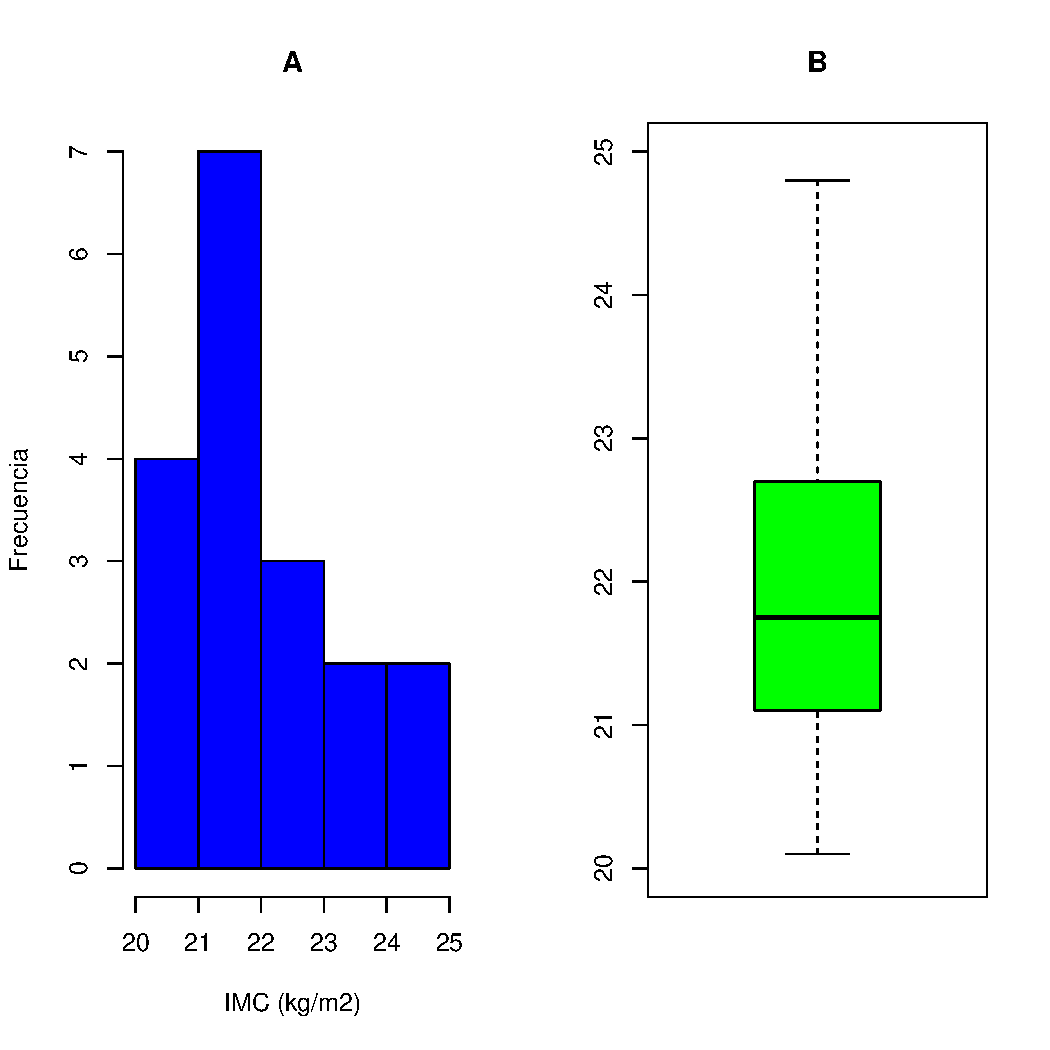
\includegraphics[width=\maxwidth]{figure/unnamed-chunk-3-1} 

\end{knitrout}

La distribuci\'on muestra un gr\'afico aproximadamente normal. Esto es, en forma de campana, centrada en 0 y con desviaci\'on est\'andar 1. 

\item Simular el TLC con datos de una distribuci\'on normal.\\

El teorema central del l\'imite establece que $\~X-\µ/(s/sqrt(n))$ que tiende a N(0,1)

\begin{itemize}
  \item \textbf{Ejemplo 2:}
\end{itemize}
Suponga que $X_i$ es normal con media $\µ=5$ y desviaci\'on est\'andar $s=5$. Entonces necesitamos una funci\'on para encontrar el valor de $\~X-\µ/(s/sqrt(n))$ 
\begin{knitrout}
\definecolor{shadecolor}{rgb}{0.969, 0.969, 0.969}\color{fgcolor}\begin{kframe}
\begin{alltt}
\hlstd{simulNorm} \hlkwb{<-} \hlkwa{function}\hlstd{(}\hlkwc{mu}\hlstd{,}\hlkwc{sigma}\hlstd{,} \hlkwc{m}\hlstd{=}\hlnum{5}\hlstd{,} \hlkwc{n}\hlstd{=}\hlnum{100}\hlstd{)}
\hlstd{\{}
\hlstd{vectMedias} \hlkwb{<<-} \hlkwd{numeric}\hlstd{(}\hlnum{0}\hlstd{)}
\hlstd{MediasEstand} \hlkwb{<<-} \hlkwd{numeric}\hlstd{(}\hlnum{0}\hlstd{)}
\hlkwa{for} \hlstd{(i} \hlkwa{in} \hlnum{1}\hlopt{:}\hlstd{m)}
\hlstd{\{}
\hlstd{X} \hlkwb{=} \hlkwd{rnorm}\hlstd{(n, mu, sigma)}
\hlcom{# genera n valores normales }
\hlstd{vectMedias[i]} \hlkwb{<<-} \hlkwd{mean}\hlstd{(X)}
\hlstd{MediasEstand[i]} \hlkwb{<<-} \hlstd{(vectMedias[i]} \hlopt{-} \hlstd{mu)}\hlopt{/}\hlstd{(sigma}\hlopt{/}\hlkwd{sqrt}\hlstd{(n))}
\hlstd{\}}
\hlstd{\}}
\hlstd{mu}\hlkwb{=}\hlnum{5}\hlstd{; sigma}\hlkwb{=}\hlnum{5}
\hlstd{m} \hlkwb{<-} \hlnum{200}
\hlcom{# número de muestras o medias a obtener }
\hlkwd{simulNorm}\hlstd{(mu, sigma, m)}
\hlkwd{hist}\hlstd{(MediasEstand,} \hlkwc{main}\hlstd{=}\hlstr{"Histograma de medias estándarizadas"}\hlstd{,}
\hlkwc{xlab}\hlstd{=}\hlstr{"Valores de m medias normales estándarizadas"}\hlstd{,}
\hlkwc{prob}\hlstd{=}\hlnum{TRUE}\hlstd{,} \hlkwc{col}\hlstd{=}\hlstr{"darkolivegreen3"}\hlstd{)}
\hlkwd{curve}\hlstd{(}\hlkwd{dnorm}\hlstd{(x,} \hlnum{0}\hlstd{,} \hlnum{1}\hlstd{),} \hlkwc{col} \hlstd{=} \hlstr{"deeppink3"}\hlstd{,} \hlkwc{lty}\hlstd{=}\hlnum{2}\hlstd{,} \hlkwc{lwd}\hlstd{=}\hlnum{2}\hlstd{,} \hlkwc{add}\hlstd{=}\hlnum{TRUE}\hlstd{)}
\end{alltt}
\end{kframe}
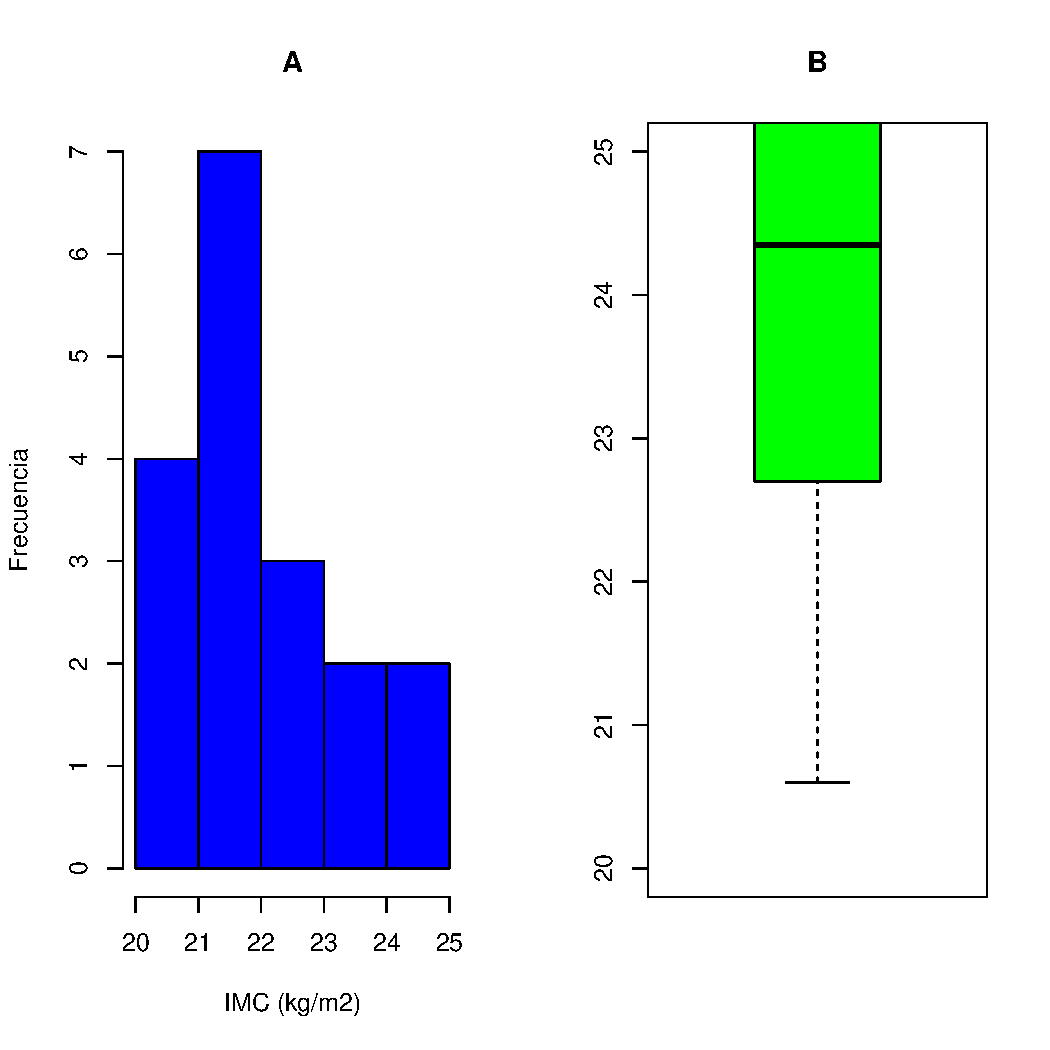
\includegraphics[width=\maxwidth]{figure/unnamed-chunk-4-1} 

\end{knitrout}

\item Un mejor gr\'afico que el histograma para decidir si los datos aleatorios son aproximadamente normal es el llamado gr\'afico de "probabilidad normal". La idea b\'asica es graficar los cuantiles de sus datos contra los correspondientes cuantiles de la distribuci\'on normal. Los cuantiles de un conjunto de datos preferidos son la Mediana, $Q_1$ y $Q_3$ los m\'as generales. El cuantil q es el valor en los datos donde q*100\%. Tambi\'en el cuantil 0.25 es $Q_1$, el cuantil 0.5 es la mediana y el cuantil 0.75 es $Q_3$. Los cuantiles para la distribuci\'on te\'orica son similares, s\'olo cambia el n\'umero de puntos datos menores, o sea el \'area a la izquierda del monto especificado. Por ejemplo, la mediana parte el \'area por debajo de la curva de densidad en la mitad.\\

El gr\'afico de probabilidad normal es f\'acil de leer si conoce c\'omo. Esencialmente, si el gr\'afico parece una l\'inea recta entonces los datos son aproximadamente normal. Est\'a l\'inea no es una l\'inea de regresi\'on. La l\'inea es trazada a trav\'es de los puntos formados por el primer y tercer cuartil.

R hace todo esto f\'acil con las funciones qqnorm(), m\'as generalmente qqplot(), y qqline() la cual traza una l\'inea de referencia (no una l\'inea de regresi\'on).
\begin{knitrout}
\definecolor{shadecolor}{rgb}{0.969, 0.969, 0.969}\color{fgcolor}\begin{kframe}
\begin{alltt}
\hlkwd{qqnorm}\hlstd{(MediasEstand,} \hlkwc{main}\hlstd{=}\hlstr{"X ~ N(0, 1)"}\hlstd{)}

\hlcom{#muestra la l\textbackslash{}'inea}

\hlkwd{qqline}\hlstd{(MediasEstand,} \hlkwc{lty}\hlstd{=}\hlnum{1}\hlstd{,} \hlkwc{lwd}\hlstd{=}\hlnum{2}\hlstd{,} \hlkwc{col}\hlstd{=}\hlstr{"red"}\hlstd{)}
\end{alltt}
\end{kframe}
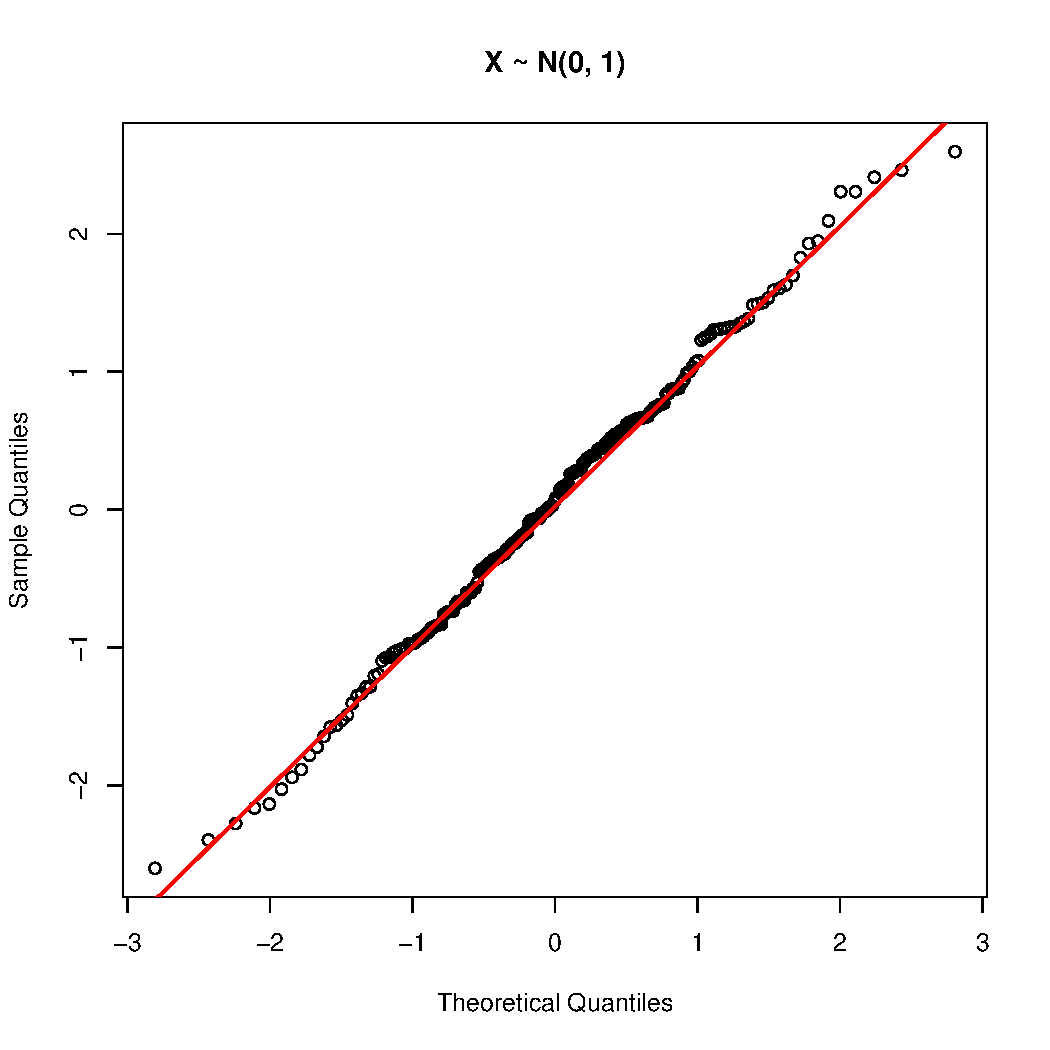
\includegraphics[width=\maxwidth]{figure/unnamed-chunk-5-1} 

\end{knitrout}

\item Simular el Teorema del L\'imite Central con datos exponencial\\
Un ejemplo de una distribuci\'on sesgada es la exponencial. Necesitamos conocer que s\'i tiene media $\µ=10$, entonces la desviaci\'on est\'andar $s$ es tambi\'en 10, por eso s\'olo necesitamos especificar la media.\\

Vamos a simular para varios valores de n. Para cada una de las m=100 muestras, n ser\'a 1, 5, 15, 50 (el n\'umero de valores aleatorios en cada uno de los promedios).
\begin{knitrout}
\definecolor{shadecolor}{rgb}{0.969, 0.969, 0.969}\color{fgcolor}\begin{kframe}
\begin{alltt}
\hlstd{simulExp} \hlkwb{<-} \hlkwa{function}\hlstd{(}\hlkwc{mu}\hlstd{,} \hlkwc{m}\hlstd{=}\hlnum{5}\hlstd{,} \hlkwc{n}\hlstd{=}\hlnum{100}\hlstd{)}
\hlstd{\{}
\hlstd{razon} \hlkwb{<-} \hlnum{1}\hlopt{/}\hlstd{mu}
\hlstd{vectMedias} \hlkwb{<<-} \hlkwd{numeric}\hlstd{(}\hlnum{0}\hlstd{)}
\hlstd{MediasEstand} \hlkwb{<<-} \hlkwd{numeric}\hlstd{(}\hlnum{0}\hlstd{)}
\hlkwa{for} \hlstd{(i} \hlkwa{in} \hlnum{1}\hlopt{:}\hlstd{m)}
\hlstd{\{}
\hlstd{X} \hlkwb{=} \hlkwd{rexp}\hlstd{(n, razon)}
\hlcom{# genera n valores exponenciales }
\hlstd{vectMedias[i]} \hlkwb{<<-} \hlkwd{mean}\hlstd{(X)}
\hlstd{MediasEstand[i]} \hlkwb{<<-} \hlstd{(vectMedias[i]} \hlopt{-} \hlstd{mu)}\hlopt{/}\hlstd{(mu}\hlopt{/}\hlkwd{sqrt}\hlstd{(n))}
 \hlstd{\}}
\hlstd{\}}
\hlkwd{par}\hlstd{(}\hlkwc{mfrow}\hlstd{=}\hlkwd{c}\hlstd{(}\hlnum{2}\hlstd{,}\hlnum{2}\hlstd{))}

\hlcom{# para n=1 }

\hlstd{mu}\hlkwb{=}\hlnum{10}
\hlstd{m} \hlkwb{<-} \hlnum{100}\hlstd{; n} \hlkwb{<-} \hlnum{1}
\hlkwd{simulExp}\hlstd{(mu, m, n)}
\hlkwd{hist}\hlstd{(MediasEstand,} \hlkwc{main}\hlstd{=}\hlstr{"Medias Exp(10); n=1"}\hlstd{,}
     \hlkwc{xlab}\hlstd{=}\hlstr{"m medias exp estándarizadas"}\hlstd{,}
\hlkwc{prob}\hlstd{=}\hlnum{TRUE}\hlstd{,} \hlkwc{col}\hlstd{=}\hlstr{"darkolivegreen3"}\hlstd{)}
\hlstd{xvals} \hlkwb{=} \hlkwd{seq}\hlstd{(}\hlkwc{from}\hlstd{=}\hlopt{-}\hlnum{3}\hlstd{,} \hlkwc{to}\hlstd{=}\hlnum{3}\hlstd{,} \hlkwc{by}\hlstd{=}\hlnum{0.01}\hlstd{)}
\hlkwd{points}\hlstd{(xvals,} \hlkwd{dnorm}\hlstd{(xvals,} \hlnum{0}\hlstd{,} \hlnum{1}\hlstd{),} \hlkwc{col} \hlstd{=} \hlstr{"red"}\hlstd{,} \hlkwc{type}\hlstd{=}\hlstr{"l"}\hlstd{,} \hlkwc{lty}\hlstd{=}\hlnum{1}\hlstd{,} \hlkwc{lwd}\hlstd{=}\hlnum{2}\hlstd{)}

\hlcom{# para n=5}

\hlstd{n} \hlkwb{<-} \hlnum{5}
\hlkwd{simulExp}\hlstd{(mu, m, n)}
\hlkwd{hist}\hlstd{(MediasEstand,} \hlkwc{main}\hlstd{=}\hlstr{"Medias Exp(10); n=5"}\hlstd{,}
     \hlkwc{xlab}\hlstd{=}\hlstr{"m medias exp estándarizadas"}\hlstd{,}
\hlkwc{prob}\hlstd{=}\hlnum{TRUE}\hlstd{,} \hlkwc{col}\hlstd{=}\hlstr{"darkolivegreen3"}\hlstd{)}
\hlstd{xvals} \hlkwb{=} \hlkwd{seq}\hlstd{(}\hlkwc{from}\hlstd{=}\hlopt{-}\hlnum{3}\hlstd{,} \hlkwc{to}\hlstd{=}\hlnum{3}\hlstd{,} \hlkwc{by}\hlstd{=}\hlnum{0.01}\hlstd{)}
\hlkwd{points}\hlstd{(xvals,} \hlkwd{dnorm}\hlstd{(xvals,} \hlnum{0}\hlstd{,} \hlnum{1}\hlstd{),} \hlkwc{col} \hlstd{=} \hlstr{"red"}\hlstd{,} \hlkwc{type}\hlstd{=}\hlstr{"l"}\hlstd{,} \hlkwc{lty}\hlstd{=}\hlnum{1}\hlstd{,} \hlkwc{lwd}\hlstd{=}\hlnum{2}\hlstd{)}

\hlcom{# Repita este proceso para n=15 y n=50}

\hlcom{# Para n=15}

\hlstd{n} \hlkwb{<-} \hlnum{15}
\hlkwd{simulExp}\hlstd{(mu, m, n)}
\hlkwd{hist}\hlstd{(MediasEstand,} \hlkwc{main}\hlstd{=}\hlstr{"Medias Exp(10); n=15"}\hlstd{,}
     \hlkwc{xlab}\hlstd{=}\hlstr{"m medias exp estándarizadas"}\hlstd{,}
\hlkwc{prob}\hlstd{=}\hlnum{TRUE}\hlstd{,} \hlkwc{col}\hlstd{=}\hlstr{"darkolivegreen3"}\hlstd{)}
\hlstd{xvals} \hlkwb{=} \hlkwd{seq}\hlstd{(}\hlkwc{from}\hlstd{=}\hlopt{-}\hlnum{3}\hlstd{,} \hlkwc{to}\hlstd{=}\hlnum{3}\hlstd{,} \hlkwc{by}\hlstd{=}\hlnum{0.01}\hlstd{)}
\hlkwd{points}\hlstd{(xvals,} \hlkwd{dnorm}\hlstd{(xvals,} \hlnum{0}\hlstd{,} \hlnum{1}\hlstd{),} \hlkwc{col} \hlstd{=} \hlstr{"red"}\hlstd{,} \hlkwc{type}\hlstd{=}\hlstr{"l"}\hlstd{,} \hlkwc{lty}\hlstd{=}\hlnum{1}\hlstd{,} \hlkwc{lwd}\hlstd{=}\hlnum{2}\hlstd{)}

\hlcom{# Para n=50}

\hlstd{n} \hlkwb{<-} \hlnum{50}
\hlkwd{simulExp}\hlstd{(mu, m, n)}
\hlkwd{hist}\hlstd{(MediasEstand,} \hlkwc{main}\hlstd{=}\hlstr{"Medias Exp(10); n=50"}\hlstd{,}
     \hlkwc{xlab}\hlstd{=}\hlstr{"m medias exp estándarizadas"}\hlstd{,}
\hlkwc{prob}\hlstd{=}\hlnum{TRUE}\hlstd{,} \hlkwc{col}\hlstd{=}\hlstr{"darkolivegreen3"}\hlstd{)}
\hlstd{xvals} \hlkwb{=} \hlkwd{seq}\hlstd{(}\hlkwc{from}\hlstd{=}\hlopt{-}\hlnum{3}\hlstd{,} \hlkwc{to}\hlstd{=}\hlnum{3}\hlstd{,} \hlkwc{by}\hlstd{=}\hlnum{0.01}\hlstd{)}
\hlkwd{points}\hlstd{(xvals,} \hlkwd{dnorm}\hlstd{(xvals,} \hlnum{0}\hlstd{,} \hlnum{1}\hlstd{),} \hlkwc{col} \hlstd{=} \hlstr{"red"}\hlstd{,} \hlkwc{type}\hlstd{=}\hlstr{"l"}\hlstd{,} \hlkwc{lty}\hlstd{=}\hlnum{1}\hlstd{,} \hlkwc{lwd}\hlstd{=}\hlnum{2}\hlstd{)}
\end{alltt}
\end{kframe}
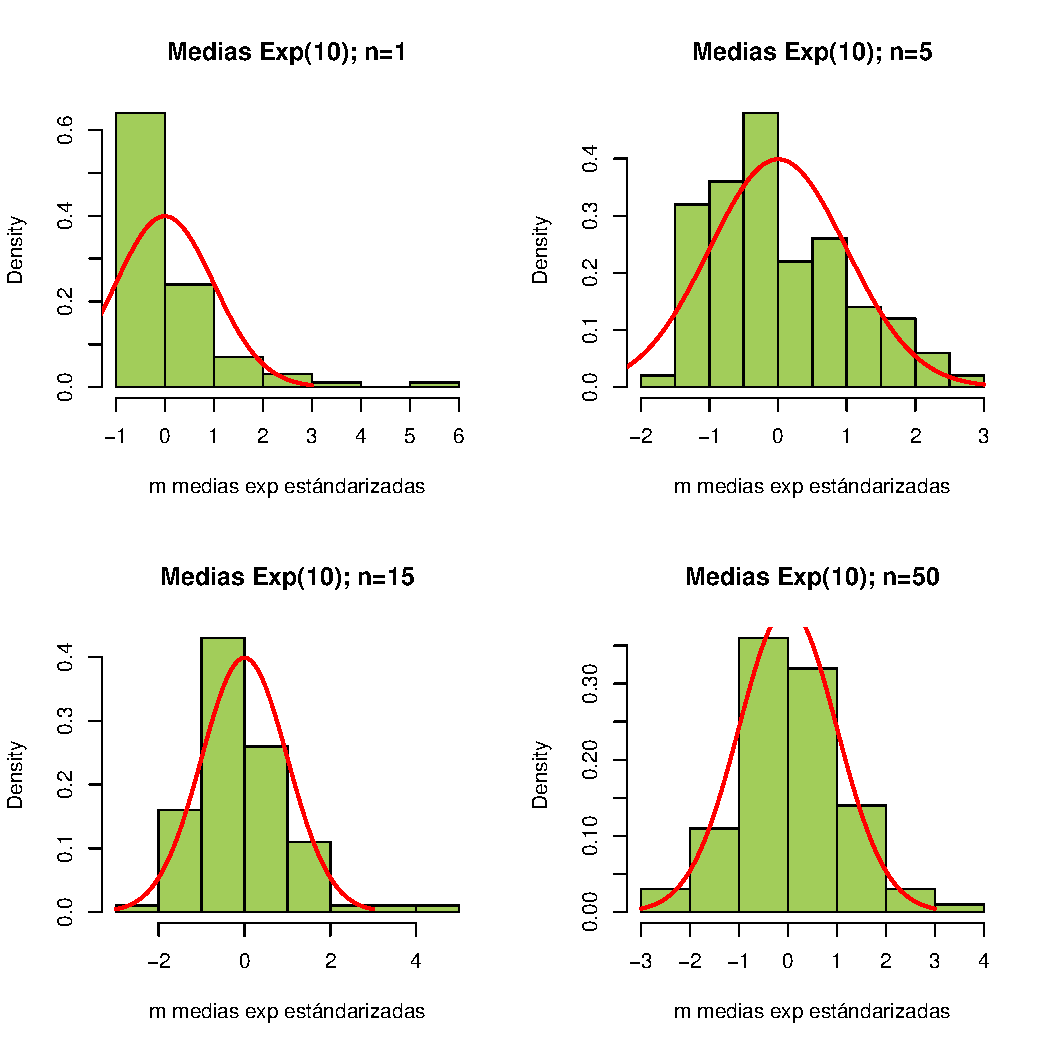
\includegraphics[width=\maxwidth]{figure/unnamed-chunk-6-1} 

\end{knitrout}

Observe que el histograma tiene una forma muy acampanada entre n=15 y n=50, aunque justo en n=50 parece todav\'ia ser un poco sesgada.\\

\textbf{Ejercicios.}
\begin{knitrout}
\definecolor{shadecolor}{rgb}{0.969, 0.969, 0.969}\color{fgcolor}\begin{kframe}
\begin{alltt}
\hlstd{simulPoiss} \hlkwb{<-} \hlkwa{function}\hlstd{(}\hlkwc{mu}\hlstd{,} \hlkwc{m}\hlstd{=}\hlnum{5}\hlstd{,} \hlkwc{n}\hlstd{=}\hlnum{100}\hlstd{)}
\hlstd{\{}

\hlstd{vectMedias} \hlkwb{<<-} \hlkwd{numeric}\hlstd{(}\hlnum{0}\hlstd{)}
\hlstd{MediasEstand} \hlkwb{<<-} \hlkwd{numeric}\hlstd{(}\hlnum{0}\hlstd{)}
\hlkwa{for} \hlstd{(i} \hlkwa{in} \hlnum{1}\hlopt{:}\hlstd{m)}
\hlstd{\{}
\hlstd{X} \hlkwb{=} \hlkwd{rpois}\hlstd{(n, mu)}
\hlcom{# genera n valores exponenciales }
\hlstd{vectMedias[i]} \hlkwb{<<-} \hlkwd{mean}\hlstd{(X)}
\hlstd{MediasEstand[i]} \hlkwb{<<-} \hlstd{(vectMedias[i]} \hlopt{-} \hlstd{mu)}\hlopt{/}\hlstd{(mu}\hlopt{/}\hlkwd{sqrt}\hlstd{(n))}
 \hlstd{\}}
\hlstd{\}}
\hlkwd{par}\hlstd{(}\hlkwc{mfrow}\hlstd{=}\hlkwd{c}\hlstd{(}\hlnum{2}\hlstd{,}\hlnum{2}\hlstd{))}

\hlcom{# para n=1 }

\hlstd{mu}\hlkwb{=}\hlnum{4}
\hlstd{m} \hlkwb{<-} \hlnum{100}\hlstd{; n} \hlkwb{<-} \hlnum{1}
\hlkwd{simulPoiss}\hlstd{(mu, m, n)}
\hlkwd{hist}\hlstd{(MediasEstand,} \hlkwc{main}\hlstd{=}\hlstr{"Medias Pois(4); n=1"}\hlstd{,}
     \hlkwc{xlab}\hlstd{=}\hlstr{"m medias exp estándarizadas"}\hlstd{,}
\hlkwc{prob}\hlstd{=}\hlnum{TRUE}\hlstd{,} \hlkwc{col}\hlstd{=}\hlstr{"darkolivegreen3"}\hlstd{)}
\hlstd{xvals} \hlkwb{=} \hlkwd{seq}\hlstd{(}\hlkwc{from}\hlstd{=}\hlopt{-}\hlnum{3}\hlstd{,} \hlkwc{to}\hlstd{=}\hlnum{3}\hlstd{,} \hlkwc{by}\hlstd{=}\hlnum{0.01}\hlstd{)}
\hlkwd{points}\hlstd{(xvals,} \hlkwd{dnorm}\hlstd{(xvals,} \hlnum{0}\hlstd{,} \hlnum{1}\hlstd{),} \hlkwc{col} \hlstd{=} \hlstr{"red"}\hlstd{,} \hlkwc{type}\hlstd{=}\hlstr{"l"}\hlstd{,} \hlkwc{lty}\hlstd{=}\hlnum{1}\hlstd{,} \hlkwc{lwd}\hlstd{=}\hlnum{2}\hlstd{)}

\hlcom{# para n=10}

\hlstd{mu}\hlkwb{=}\hlnum{4}
\hlkwd{simulPoiss}\hlstd{(mu, m, n)}
\hlkwd{hist}\hlstd{(MediasEstand,} \hlkwc{main}\hlstd{=}\hlstr{"Medias Pois(4); n=10"}\hlstd{,}
     \hlkwc{xlab}\hlstd{=}\hlstr{"m medias exp estándarizadas"}\hlstd{,}
\hlkwc{prob}\hlstd{=}\hlnum{TRUE}\hlstd{,} \hlkwc{col}\hlstd{=}\hlstr{"darkolivegreen3"}\hlstd{)}
\hlstd{xvals} \hlkwb{=} \hlkwd{seq}\hlstd{(}\hlkwc{from}\hlstd{=}\hlopt{-}\hlnum{3}\hlstd{,} \hlkwc{to}\hlstd{=}\hlnum{3}\hlstd{,} \hlkwc{by}\hlstd{=}\hlnum{0.01}\hlstd{)}
\hlkwd{points}\hlstd{(xvals,} \hlkwd{dnorm}\hlstd{(xvals,} \hlnum{0}\hlstd{,} \hlnum{1}\hlstd{),} \hlkwc{col} \hlstd{=} \hlstr{"red"}\hlstd{,} \hlkwc{type}\hlstd{=}\hlstr{"l"}\hlstd{,} \hlkwc{lty}\hlstd{=}\hlnum{1}\hlstd{,} \hlkwc{lwd}\hlstd{=}\hlnum{2}\hlstd{)}

\hlcom{# para n=30 }

\hlstd{mu}\hlkwb{=}\hlnum{4}
\hlkwd{simulPoiss}\hlstd{(mu, m, n)}
\hlkwd{hist}\hlstd{(MediasEstand,} \hlkwc{main}\hlstd{=}\hlstr{"Medias Pois(4); n=30"}\hlstd{,}
     \hlkwc{xlab}\hlstd{=}\hlstr{"m medias exp estándarizadas"}\hlstd{,}
\hlkwc{prob}\hlstd{=}\hlnum{TRUE}\hlstd{,} \hlkwc{col}\hlstd{=}\hlstr{"darkolivegreen3"}\hlstd{)}
\hlstd{xvals} \hlkwb{=} \hlkwd{seq}\hlstd{(}\hlkwc{from}\hlstd{=}\hlopt{-}\hlnum{3}\hlstd{,} \hlkwc{to}\hlstd{=}\hlnum{3}\hlstd{,} \hlkwc{by}\hlstd{=}\hlnum{0.01}\hlstd{)}
\hlkwd{points}\hlstd{(xvals,} \hlkwd{dnorm}\hlstd{(xvals,} \hlnum{0}\hlstd{,} \hlnum{1}\hlstd{),} \hlkwc{col} \hlstd{=} \hlstr{"red"}\hlstd{,} \hlkwc{type}\hlstd{=}\hlstr{"l"}\hlstd{,} \hlkwc{lty}\hlstd{=}\hlnum{1}\hlstd{,} \hlkwc{lwd}\hlstd{=}\hlnum{2}\hlstd{)}

\hlcom{# Para n=50}

\hlstd{mu}\hlkwb{=}\hlnum{4}
\hlkwd{simulPoiss}\hlstd{(mu, m, n)}
\hlkwd{hist}\hlstd{(MediasEstand,} \hlkwc{main}\hlstd{=}\hlstr{"Medias Pois(4); n=50"}\hlstd{,}
     \hlkwc{xlab}\hlstd{=}\hlstr{"m medias exp estándarizadas"}\hlstd{,}
\hlkwc{prob}\hlstd{=}\hlnum{TRUE}\hlstd{,} \hlkwc{col}\hlstd{=}\hlstr{"darkolivegreen3"}\hlstd{)}
\hlstd{xvals} \hlkwb{=} \hlkwd{seq}\hlstd{(}\hlkwc{from}\hlstd{=}\hlopt{-}\hlnum{3}\hlstd{,} \hlkwc{to}\hlstd{=}\hlnum{3}\hlstd{,} \hlkwc{by}\hlstd{=}\hlnum{0.01}\hlstd{)}
\hlkwd{points}\hlstd{(xvals,} \hlkwd{dnorm}\hlstd{(xvals,} \hlnum{0}\hlstd{,} \hlnum{1}\hlstd{),} \hlkwc{col} \hlstd{=} \hlstr{"red"}\hlstd{,} \hlkwc{type}\hlstd{=}\hlstr{"l"}\hlstd{,} \hlkwc{lty}\hlstd{=}\hlnum{1}\hlstd{,} \hlkwc{lwd}\hlstd{=}\hlnum{2}\hlstd{)}
\end{alltt}
\end{kframe}
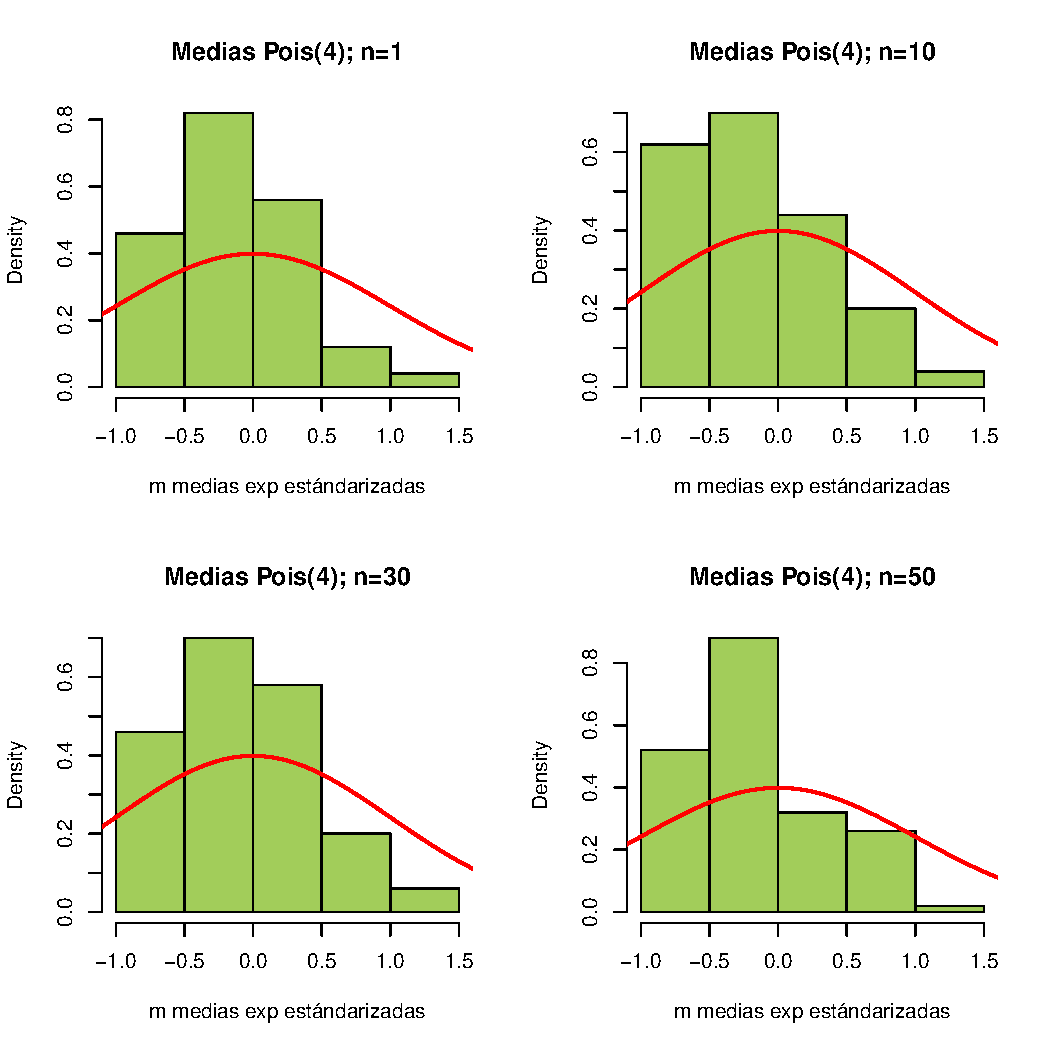
\includegraphics[width=\maxwidth]{figure/unnamed-chunk-7-1} 

\end{knitrout}




\end{enumerate}
\end{document}
